
\section{Билет 19.Принцип максимума и минимума для гармонических функций. Единственность классического решения задачи Дирихле для уравнения Пуассона при непрерывной граничной функции}
%Никитушка отмочил красоту
\subsection{Теорема (принцип максимума)}
\begin{theorem}
{\bf(Принцип максимума)} Если $u(x)$ - гармоническая в
области $\Omega$ и достигает $max$ или $min$ значения в
точке $a \in \Omega$, то $u(x) \equiv u(a) \Forall x \in \Omega$ 

\begin{offtop}
Теорема справедлива в $\R^n$
\end{offtop}

\begin{proof}

\begin{itemize}
\item
\item 
Докажем вспомогательное локальное 
\begin{statement}
\label{statement_19.1}
Пусть $u(x) \in C^2(\Omega)$ достигает максимума в точке $a$, а так же удовлетворяет {\bf свойству среднего}:

\[
u(a) = \dfrac{1}{4\pi r^2}\oint\limits_{\abs{y-a} = r}u(y
)\;dS_y \Forall r: 0 < r < d_a = dist(a, \R^3 \backslash
 \Omega)
\]

Тогда $u(x) \equiv u(a) \Forall x \in B(a, d_a)$  

\end{statement}
\begin{proof}
$
u(a) = \dfrac{1}{4\pi r^2}\oint\limits_{\abs{y-a} = r}u(y
)\;dS_y  =
\dfrac{u(a)}{4\pi r^2}\oint\limits_{\abs{y-a} = r} \;dS_y  +
 		\dfrac{1}{4\pi r^2}\oint\limits_{\abs{y-a} = r}\brs{u(y
)-u(a)}\;dS_y =
	u(a) + \dfrac{1}{4\pi r^2}\oint\limits_{\abs{y-a} = r}\brs{u(y
)-u(a)}\;dS_y \Rightarrow 
	\oint\limits_{\abs{y-a} = r}\underbrace{\brs{u(y)-u(a)}}_{\le 0,\ \text{непрерывна}}\;dS_y = 0
	 \Leftrightarrow
	\quad u(y) = u(a) \Forall y: |y-a|=r < d_a
 $
\end{proof}

\item
{\bf Докажем саму теорему}
\begin{center}
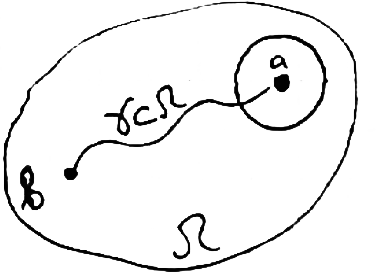
\includegraphics[scale=0.5]{19_1_new}
\end{center}
Соединим $a$ и $b$ кусочно-гладкой кривой. Эту кривую параметризуем натуральным параметром(параметризация кривой длиной её дуги): 
$x = x(s), x(0) = a, x(L) = b$.
{\bf Обозначим}
$d = dist\fbrs{\gamma = x; \partial{\Omega}} > 0$
($d$ действительно $> 0$ : если $d = 0$, то 
$\exists\{x_n\}_{n=1}^\infty \subset \gamma: \rho\brs{x_n, \partial\Omega}\to 0$.
 Выделим из $\{x_n\}$ сходящуюся $\{x_{n_k}\}=\{y_k\}$($\gamma$ - ограничено). Пусть $y_k \to y_0$. Тогда $y_0$ - предельная для
 $\partial \Omega$ в силу замкнутости 
 $y_0 \in \gamma \cup \partial \Omega \Rightarrow$ противоречие)\\
 Разобьем $[0,L]$ на части размера $\Delta S = \dfrac{L}{N}$\\
 Пусть $\fbrs{S_k = k\Delta S, x_k = x(S_k)}$. 
 Число N выберем так, чтобы $\Delta S = \dfrac{L}{N} < d$\\
 \begin{center}
 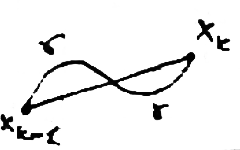
\includegraphics[scale=0.5]{19_2_new}
 \end{center}
 Заметим, что $\abs{x_k - x_{k-1}} \boxed{\leq} s_k - s_{k-1} < d$($\boxed{\cdot}$ - кратчайшее расстояние между точками это отрезок).
 \begin{center}
 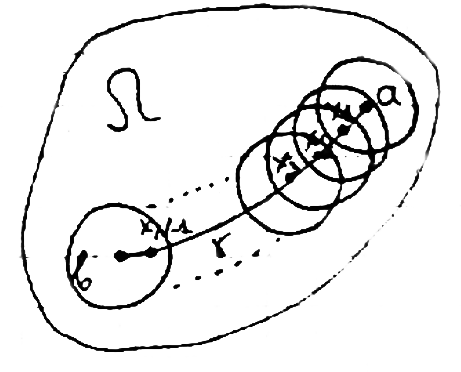
\includegraphics[scale=0.5]{19_3_new}
\end{center}
 Рассмотрим шары ${B_d(x_k)}_{k=0}^N$. В силу
 $\abs{x_k - x_{k-1}}) < d$ верно $x_{k+1} \in B_d(x_k)$. 
  Примем утверждение \ref{statement_19.1} к первому шару. 
  Как следствие $u(x_1) = u(a)\Rightarrow$ утверждение \ref{statement_19.1} применимо уже ко второму шару.
   В цепочке шаров конечное число 
  $\Rightarrow$ добираемся до точки $b$ - теорема доказана.  
\end{itemize}
\end{proof}
\end{theorem}

$\bullet$ Заметим, что достаточно было потребовать
свойство среднего и непрерывность, вместо гармоничности.


\begin{conseq}
\label{conseq19.1}
Пусть $\Omega$ - ограниченная область, а $u(x)$ - гармоническая в $\Omega$ и непрерывная на $\overline{\Omega}$.
Тогда $u(x)$ достигает $max$ и $min$ на $\partial \Omega$, т.е.
$\min\limits_{y \in \partial \Omega}u(y) \leq u(x) \leq \max\limits_{y \in \partial \Omega}u(y)$
	\begin{proof}
	Либо максимум/минимум на границе, либо $u(x)\equiv const$ в $\Omega$
	\end{proof}
\end{conseq}


\begin{conseq}
Для указанной в следствии \ref{conseq19.1} $u(x) \hookrightarrow \abs{u(x)} \leq \max\limits_{y \in \partial \Omega} \abs{u(y)}$
\begin{proof}

\begin{equation}
  \begin{cases}
  & u(x) \leq \max\limits_{\partial \Omega}u(y) \leq \max\limits_{\partial \Omega}\abs{u(y)}\\  
  &-u(x) \leq \max\limits_{\partial \Omega}(-u(y)) \leq \max\limits_{\partial \Omega}\abs{u(y)}\\
  \end{cases}
  \end{equation}  
  
  $\Rightarrow \abs{u(x)} \leq \max\limits_{\partial \Omega}\abs{u(y)}$
\end{proof}
\end{conseq}


\subsection{Новая постановка задачи Дирихле для уравнения Пуассона}
$\Omega$ - ограниченная область 

\begin{equation}
  \begin{cases}\label{equatation19.1}
  & \Delta u(x) = f(x), x \in \Omega\\ 
  & \while{u(x)}{\partial \Omega} = u_0(x), x \in \partial \Omega\\
  \end{cases}
\end{equation} 
  
 \begin{definition}
 Классическое решение задачи Дирихле - функция
  $u(x) \in C^2(\Omega) \cap C(\overline{\Omega})$,
  удовлетворяющая уравнению и граничному условию.(раньше было $u(x) \in C^2(\Omega) \cap C^{\boxed{1}}(\overline{\Omega})$, единица была нужна для формул Грина, теперь убираем ее)
 \end{definition}
 \subsection{Теорема единственности}
 \begin{theorem}
 (единственности) Не может существовать более 1 классического решения задачи Дирихле(\ref{equatation19.1}).
 
 \begin{proof}
 Пусть $u_1$ и $u_2$ - классические решения (\ref{equatation19.1}). Тогда $v(x) = u_1 - u_2$ - классическое решение полностью однородной задачи:
 
 \begin{equation}
  \begin{cases}\label{equatation19.2}
  & \Delta v(x) \equiv 0, x \in \Omega\\ 
  & \while{v(x)}{\partial \Omega} = 0, x \in \partial \Omega\\
  \end{cases}
\end{equation}
 
 Согласно принципу максимума, $\abs{v(x)} \leq \max\limits_{\partial\Omega} \abs{v(x)} = 0 \Rightarrow v(x) \equiv 0$
 \end{proof}
 \end{theorem}